Целью работы стало написание модуля для программного комплекса. Модуль выполняет проверку файлов-изображений на их подлинность (являются ли они действительно изображением), и выводить информацию в формате XML.

\subsubsection{Реализация программного модуля}
Сначала необходимо было узнать, как различать изображения и файлы с расширением изображений. Было принято решение считывать заголовки файлов и сравнивать их с корректными заголовками, являющимися уникальными для соответствующего формата. Далее была найдена информация о заголовках нескольких форматов. Форматы заголовков представлены в таблице~\ref{tab:formats}.

% таблица форматов заголовков
\begin{table}[ht]
\caption{Форматы заголовков}
\label{tab:formats}
\begin{center}
\begin{tabular}{|p{8cm}|p{9cm}|}
\hline
Формат & Заголовок \\
\hline
JPEG & FFD8 \\
\hline
PNG & 89504E47 \\
\hline
GIF & 474946 \\
\hline
BMP & 424D \\
\hline
TIFF & 49492A \\
\hline
\end{tabular}
\end{center}
\end{table}

Также было принято решение проверять на корректность конец файла, так как к изображению можно прикрепить архив в конец файла. На данный момент реализована проверка конца файла для форматов JPEG и PNG как самых популярных и простых для реализации (табл.~\ref{tab:ends}).

% таблица форматов конца файла
\begin{table}[ht]
\caption{Форматы конца файла}
\label{tab:ends}
\begin{center}
\begin{tabular}{|p{8cm}|p{9cm}|}
\hline
Формат & Конец \\
\hline
JPEG & FFD9 \\
\hline
PNG & AE426082 \\
\hline
\end{tabular}
\end{center}
\end{table}

\subsubsection{Алгоритм работы модуля}
Алгоритм программы, проверяющей заголовки и концы файлов, представлен на рисунке~\ref{block_ilya:block_ilya}.

\begin{figure}[h!]                                          % тут рисунок block_ilya
\center{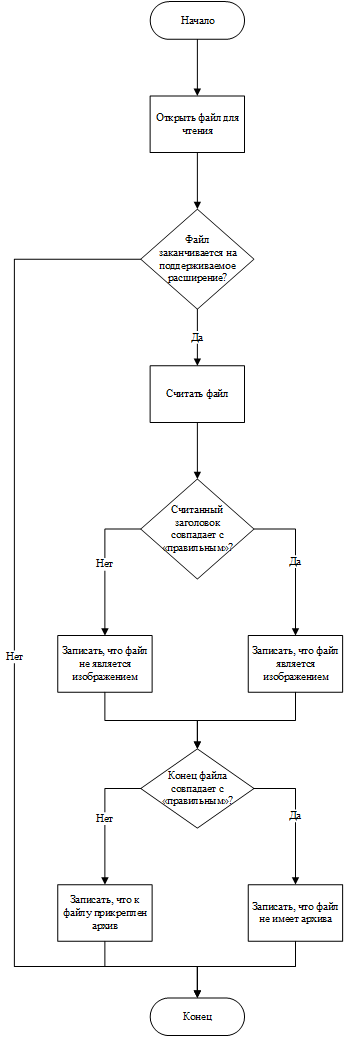
\includegraphics[scale=0.9]{block_ilya}}
\caption{Блок-схема алгоритма программы, проверяющей заголовки и концы файлов}
\label{block_ilya:block_ilya}
\end{figure}

\subsubsection{Структура XML-файла}
Файл начинается с пролога, описывающего версию XML и кодировку. Далее идет начальный элемент <add>, а для каждого изображения создается элемент <doc>. В теле <doc> записаны поля <field name>value</field>, далее закрывается элемент </doc>, а в конце документа находится конечный элемент </add>.

Пример структуры XML-файла представлен на рисунке~\ref{xml_ilya:xml_ilya}.

\begin{figure}[h!]                                          % тут рисунок xml_ilya
\center{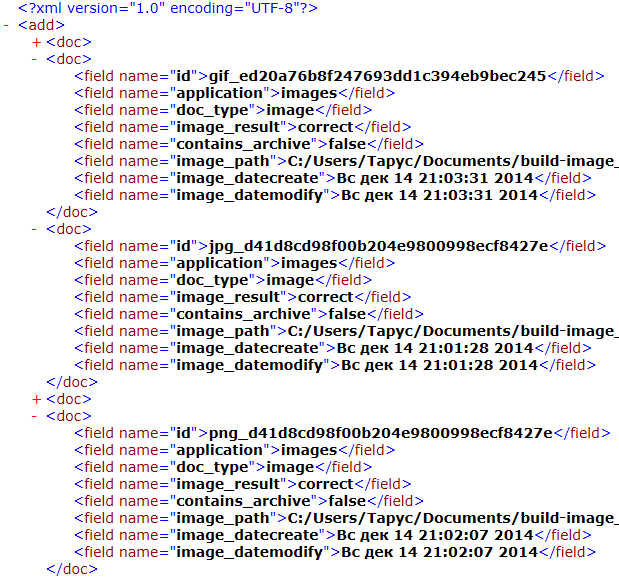
\includegraphics[width=0.6\linewidth]{xml_ilya}}
\caption{Структура XML-файла}
\label{xml_ilya:xml_ilya}
\end{figure}

Значение поля id --- «формат изображения»\_«MD5 сумма от файла».
Поля image\_result и contains\_archive непосредственно указывают на то, является ли файл изображением, и прикреплен ли к нему архив соответственно. Также имеется полный путь до файла, дата создания и дата изменения.
В программу были введены следующие тесты: 5 файлов изображений для базовой проверки, 5 текстовых файлов с расширением изображений, и 2 файла изображений с прикрепленным к ним архивам. Все файлы программа распознала корректно и вывела в XML файл.


Библиотеки Qt, использованные для написания программного модуля:
\begin{itemize}
\item QFile --- для открытия и чтения всего файла;
\item QString --- для работы со строками в программе;
\item QDebug --- для вывода в консоль в целях отладки;
\item QDataStream --- для считывания отдельных байтов из потока;
\item QXmlStreamWriter --- для вывода в XML;
\item QFileInfo --- для считывания информации о файле (даты и т.д.);
\item QDateTime --- для работы с форматом даты, в который записывается информация о файле;
\item QCryptographicHash --- для получение md5 суммы.
\end{itemize}


Результат работы программы представлен на рисунке~\ref{result_ilya:result_ilya}.

\begin{figure}[ht]                                          % тут рисунок result_ilya
% \center{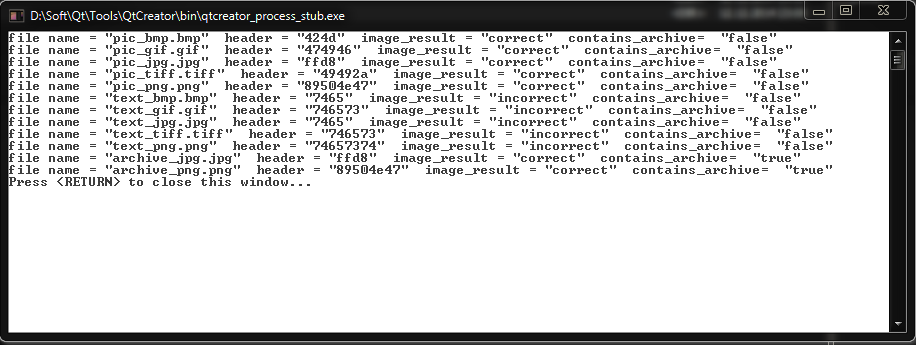
\includegraphics[width=0.6\linewidth]{result_ilya}}
\center{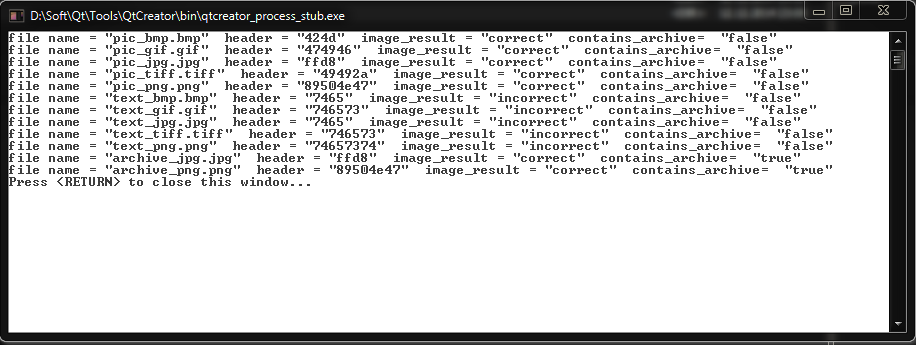
\includegraphics[scale=0.7]{result_ilya}}
\caption{Результат работы программы}
\label{result_ilya:result_ilya}
\end{figure}

\subsubsection{Задачи на следующий семестр}
В будущем в программе будут реализованы:
\begin{itemize}
\item  поддержка новых расширений;
\item  возможность проверить наличие архива для всех расширений;
\item  рекурсивный обход директорий.
\end{itemize}

\clearpage

